\section{Experimental Evaluation}
\label{sec:eval}

%Opening is deliberately short because we gonna be running out of space 
In this section, we present empirical and analytical evaluation of the performance and cost of \sysname under different workloads and scales. 
Our evaluation consists of empirical analysis of the different scientific computing applications, as well as model-driven simulations for analyzing and comparing \sysname behavior under different preemption and application dynamics. 

% \begin{itemize}
% \item What is performance and cost of 
% \end{itemize}

\noindent \textbf{Environment and Workloads:} All our empirical evaluation is conducted on the Google Public Cloud, and with these representative scientific applications: 
% open-source
\vspace*{\tightext}
\begin{description}
  %TODO: Need MAX two sentence descriptions
\item[NC.] The ions in nanoconfiment~\cite{} application computes dynamics of nanoparticles. Uses OpenMP and MPI parallelization. 
\item[Shapes.]  Application to compute shapes of nanoparticles. Uses OpenMP and MPI parallelization and is embarrassingly parallel. 
\item[Lulesh.] Popular hydrodynamics application with the default parameters. 
\end{description}
\vspace*{\tightext}
All applications use OpenMPI, are deployed on Slurm vXXX and 64-bit Ubuntu 18.04, and run on Google Cloud VMs with x86-64 Intel Broadwell CPUs. 
%Networking? 


\subsection{SciSpot Performance and Cost}

\noindent \textbf{Impact of server exploration.}
As described in Section~\ref{sec:design}, applications can be deployed on multiple types of VMs in the cloud, with each VM type having a different number of CPUs. 
Figure~\ref{fig:runtimes-bar} shows the running times of the different applications 


\begin{figure}
  \centering
  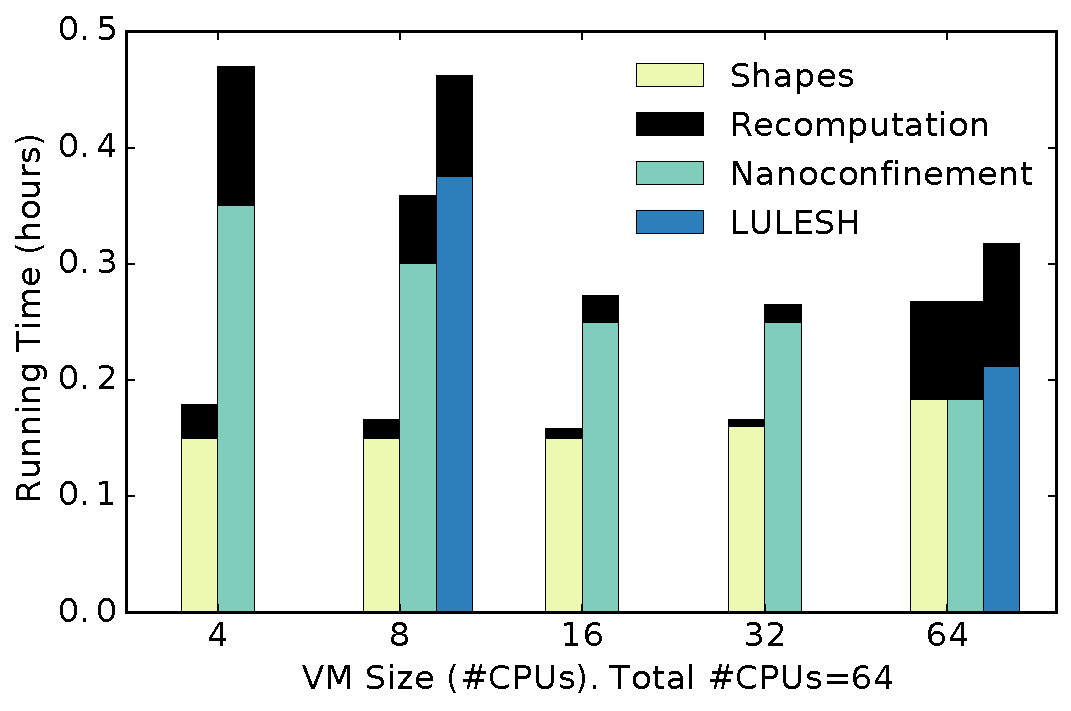
\includegraphics[width=0.4\textwidth]{../graphs/runtime-bars.pdf}
  \caption{Running times of applications on different servers}
  \label{fig:runtimes-bar}
\end{figure}


\noindent \emph{ \textbf{Result:} Selecting the right server type can have big impact on application performance. The increase in running time due to recomputation is small and less than 5\%.}


\noindent \textbf{Cost.} Using preemptible VMs results in significant lower costs, even considering the increase in running time and cost due to the preemptions.
\sysname's server selection 



\begin{figure}
  \centering
  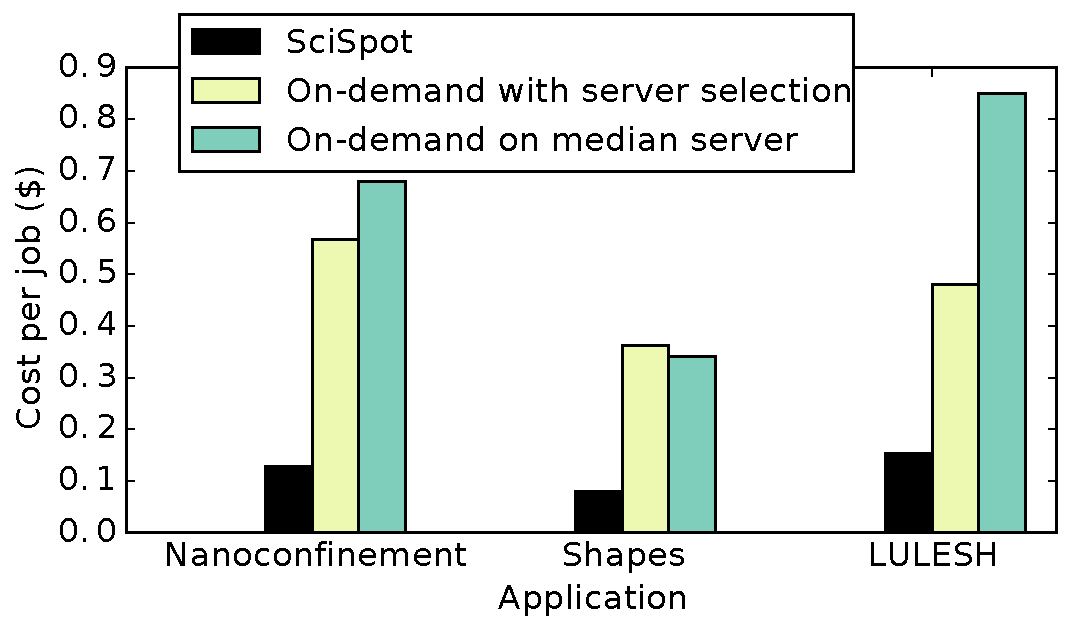
\includegraphics[width=0.4\textwidth]{../graphs/cost-only-bar.pdf}
  \caption{Cost of different configurations}
  \label{fig:cost-only-bar}
\end{figure}

\noindent \emph{ \textbf{Result:} SciSpot reduces computing costs by up to 5x and 7x compared to on-demand cloud servers.}


\noindent \textbf{Comparison with HPC Clusters:}

\begin{figure}[t]
  \centering 
  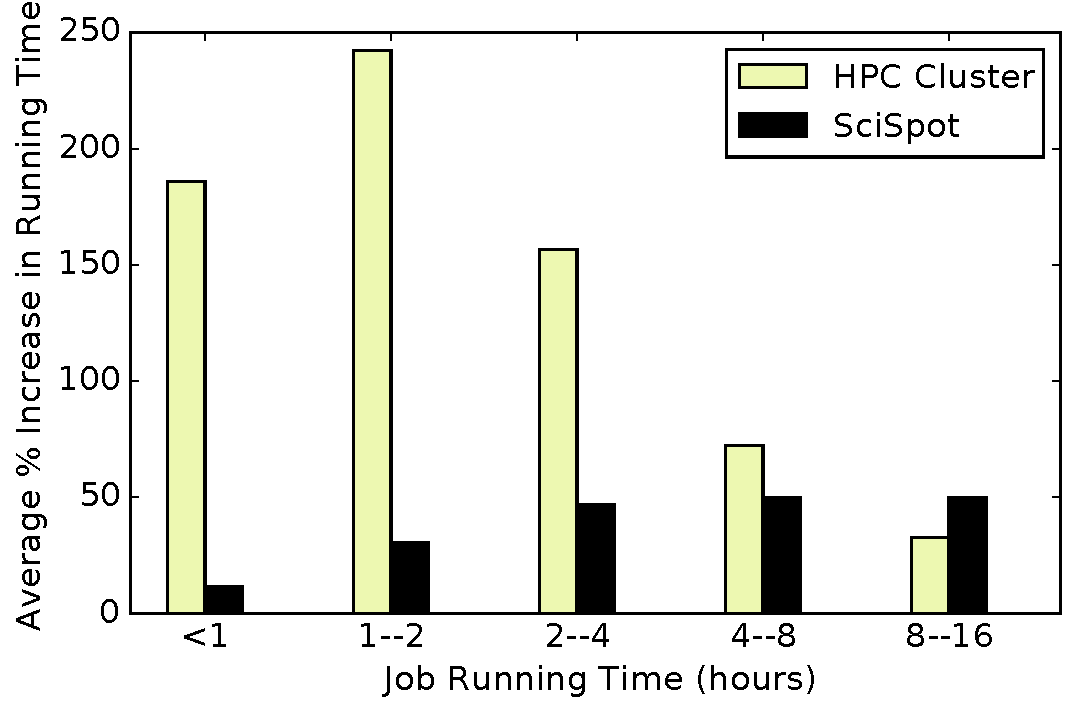
\includegraphics[width=0.4\textwidth]{../graphs/hpc-vs-scispot.pdf}
  \caption{HPC vs SciSpot overhead}
  \label{fig:hpc-vs-scispot}

\end{figure}

\noindent \emph{ \textbf{Result:} While preemptions can increase running times due to recomputation, this increase is small, and is between 20 to 400\% lower compared to conventional HPC clusters. }


\subsection{SciSpot Scaling}


\begin{figure}
  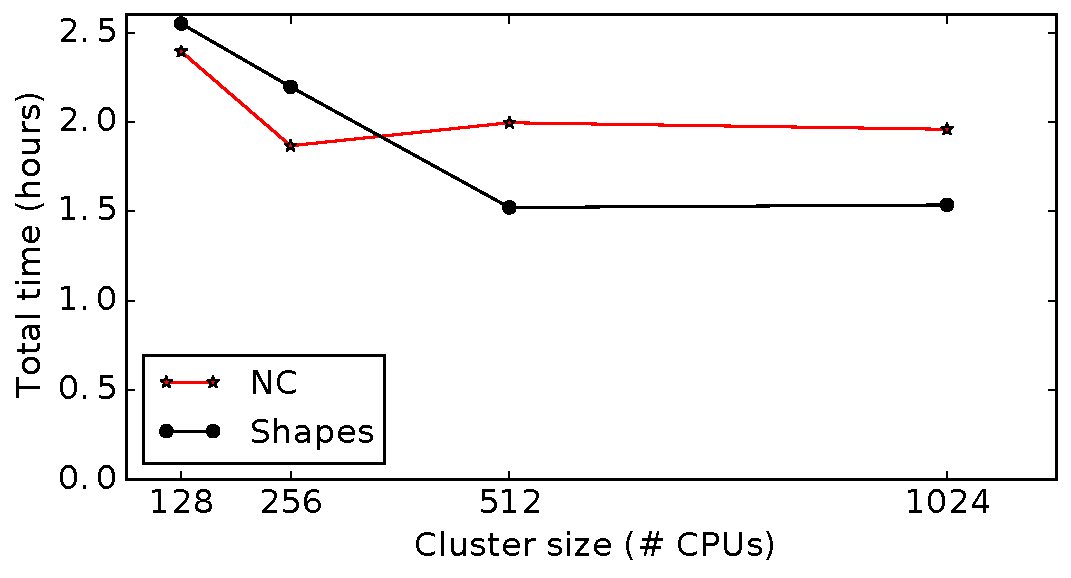
\includegraphics[width=0.4\textwidth]{../graphs/vm-per-job-scaling.pdf}
  \caption{SciSpot scaling as the VMs per jobs increases}
  \label{fig:vm-per-job-scaling}
\end{figure}

Figure~\ref{fig:vm-per-job-scaling} shows the total bag of job execution times for 32 jobs with 4 jobs running in parallel.
32 CPU VM's were used, and thus the total number of CPUs = 32*jobs-per-VM. Max CPU's used was 512 
Reach saturation because of the limitations of parallel speedup and coordination. 


\begin{figure}
  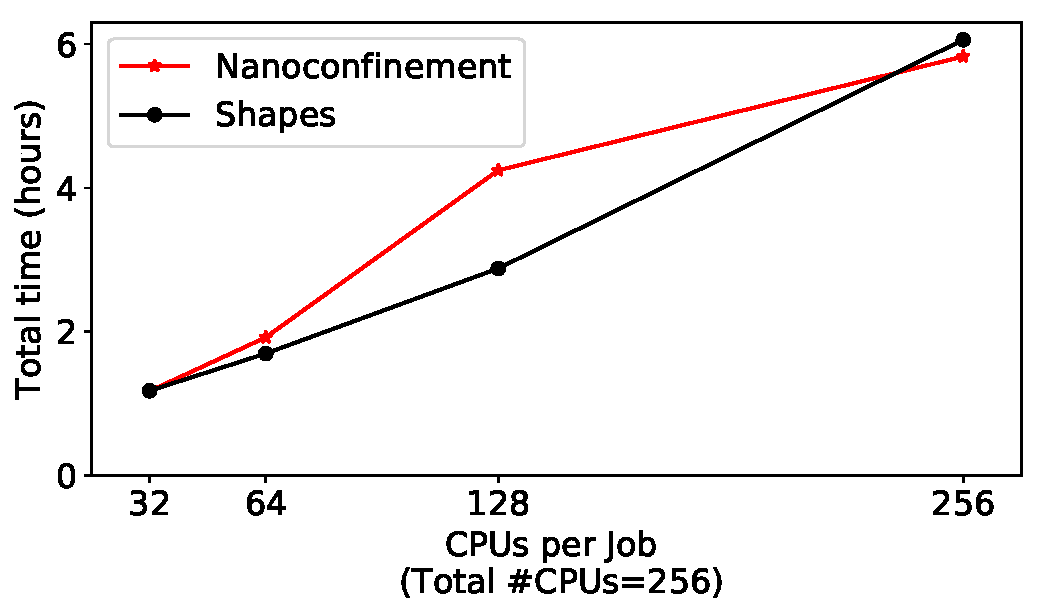
\includegraphics[width=0.3\textwidth]{../graphs/par-scaling.pdf}
  \caption{Job running times as the CPU's per job increases}
  \label{fig:par-scaling}
\end{figure}

Figure~\ref{fig:par-scaling} shows the running time when the total cluster size is fixed, but the number of parallel jobs and hence the number of CPUs per job changes. Smaller number of CPUs extracts higher parallel speedup and is thus recommended.


\noindent \textbf{Impact of Preemptions:} Figure~\ref{fig:fails-time} shows the total running time of the bag of jobs (32 jobs) for the nanoconfiment workload, when the total cluster size is 4 VMs. We ran the workload multiple times with different number of VM preemptions and hence jobs that failed. We see that even with a high number of preemptions, the running time only increases by about 30\%.
We note that this happens with a vanishingly small likelihood, for instance when the demand is very high and the preemptible VMs see high failure rates.
This shows that \sysname is robust and can provide acceptable performance even under extreme, adverse conditions. 

\begin{figure}[t]
  \centering 
  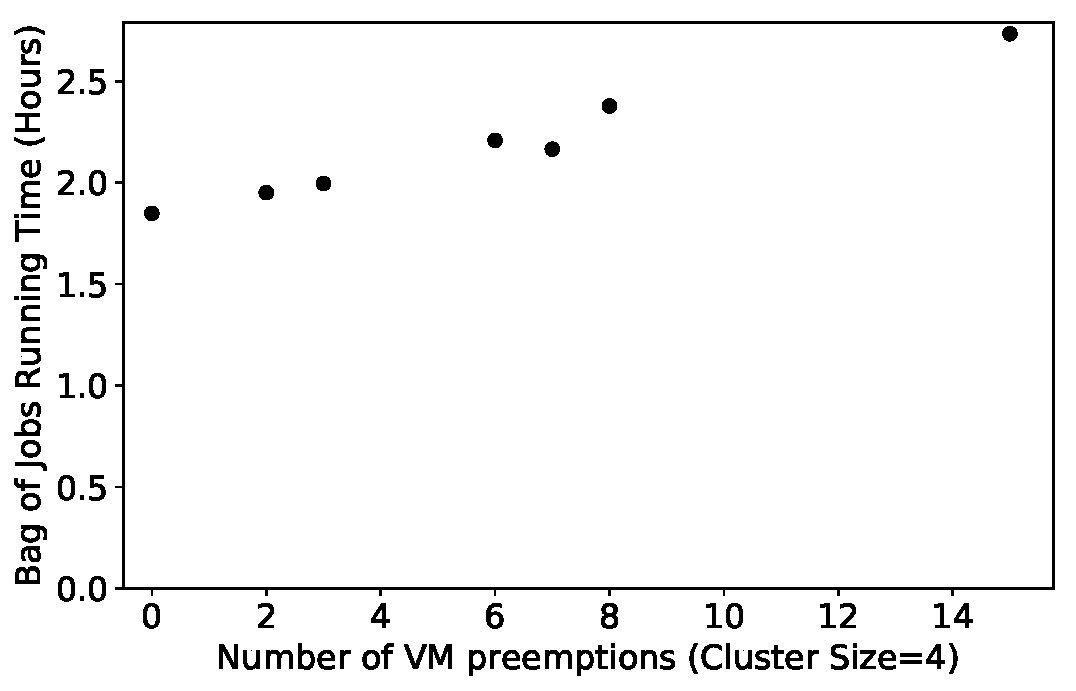
\includegraphics[width=0.4\textwidth]{../graphs/confin-fails-vs-time.pdf}
  \caption{The running time of a bag of 32 jobs increases by less than 40\%, even when the number of preemptions is high.}
  \label{fig:fails-time}
\end{figure}

\noindent \textbf{Large Bags:} Essentially time scalability. 4 Jobs in Parallel, each with 2 VMs each.  

%32_2_4 
\begin{table}
  \begin{tabular}{|c|r|r|}
    \hline
    Workload & Jobs & Time (Hours) \\
    \hline
    NC & 32  & 112 \\
    NC & 100  & 365 \\
    \hline
    Shapes & 32 & 88 \\
    Shapes & 100 & 269 \\  
    \hline
  \end{tabular}
  \caption{Running time for large, long-running bags of jobs.}
  \label{tab:100-jobs}
\end{table}



% \begin{figure}
%   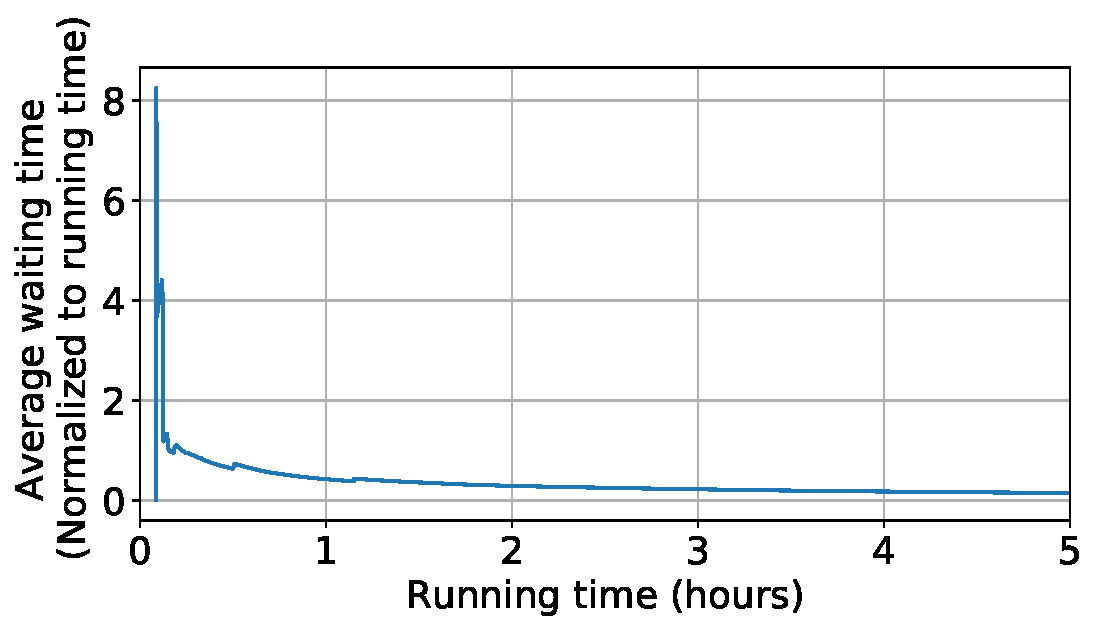
\includegraphics[width=0.4\textwidth]{../data/waiting_cumul.pdf}
%   \caption{The average waiting time (normalized to running time) of jobs of different length.}
%   \label{fig:hpc-wait-cdf}
% \end{figure}



%%% Local Variables:
%%% mode: latex
%%% TeX-master: "paper"
%%% End:
